%%%%%%%%%%%%%%%%%%%%%%%%%%%%%%%%%%%%%%%
%%%%%   STATISTICAL METHODOLOGY   %%%%%
%%%%%%%%%%%%%%%%%%%%%%%%%%%%%%%%%%%%%%%
\chapter{Statistical methodology}
\label{ch:3.0}

%Mathematical modelling and its analyses have been central to the understanding of infectious diseases in epidemiology. 
The statistical approaches used throughout the thesis are introduced in this chapter.
Section \ref{sec:sampling.distribution} describes the sampling distribution.
All the different sets of stochastic models applied to the data 
%and its statistical principles %used to apply to such data being 
are introduced in Section \ref{sec:models}, and finally, the %basic terminology and fundamental concept
methods used 
%in the field of mathematical modelling of infectious disease dynamics and its transmission are 
for parameter estimation, the approaches used to estimate confidence intervals, models evaluation, and selection, are described in Section \ref{sec:inference}.
%where the principal statistical methods used throughout the thesis for parameter estimation, model evaluation and selection, and inference are explained.
%Since no model can serve all purposes equally well.\textbf{[book - modelling parasite transmission and control]}\\
%In modelling malaria, it is useful to conduct studies that build a broad range of models and that explicitly consider the question of robustness of a model. \textbf{[book - modelling parasite transmission and control]}



%%%%%%%%%%%%%%%%%%%%%%%%%
% SAMPLING DISTRIBUTION %
%%%%%%%%%%%%%%%%%%%%%%%%%
\section{Sampling distribution}
\label{sec:sampling.distribution}

%As previously described in Chapter \ref{ch:2.0}, 
%The data set analysed was created from a cross-sectional study, with the variables registered through single screenings amongst all villages \cite{drakeley2005estimating}.
%The fundamental assumption in order to to apply stochastic methodologies to a cross-sectional data set is to consider individuals' age as proxy for time of exposure.
%By not having follow up data, the key assumption in order to estimate malaria transmission intensity through stochastic methodologies is to  
%This assumption allows to create a measure for historical exposure based on the sequence of the sampled population's age, as one infers older individuals are more likely to have been exposed to malaria parasites \cite{keeling2009mathematical}.
For the data collection in the original study \cite{drakeley2005altitude}, the selected individuals were screened for the presence malaria parasites and three specific \textit{P. falciparum} malarial antigens (MSP1, MSP2, and AMA1).
Each individual was recorded as infected or not infected for malaria, and seropositive or seronegative for the different antigens.
Within each village, the study design placed all sampled individuals in three distinct age groups with defined ranges $[1,5)$, $[5,15)$, and $[15,46)$, each one representing a specific percentage of the %total sampled
recorded population (example of village structure in Table \ref{tab:multinomial.bwambo}).
Under this structured data, the objective of the thesis is then to infer about the number of individuals with status infected/seropositive.

Since the total number of individuals placed within each age group $g=(1,2,3)$ is known, one can assume that the random vector containing the number of
individuals with each combination of characteristics (exact age $i=(I_{g_{min}},\dots,I_{g_{max}})$ and infection or seropositivity status, $j=(0,1)$) follows a Multinomial distribution, where $I_{g_{min}}$ and $I_{g_{max}}$ represent the minimum and the maximum exact ages in age group $g$.
Let $\tilde{X}$ be such vector.
For easiness of reading we shall refer to $\tilde{X}$ as $\tilde{X}_{gij}$ so that track of indexes is kept.
Let $\tilde{x}_{gij}$ be the observed vector and $x_{gij}$ represent the number of individuals in age group $g$, exact age $i$, and status $j$.
The vector $\tilde{x}_{gij}$ is then presented in Table \ref{tab:multinomial.bwambo} with three groups of rows ($g=(1,2,3)$), each with the distribution of the positive and negative cases ($j=(0,1)$) for all the ages within the age group ($i=(I_{g_{min}},\dots,I_{g_{max}})$).
% \textcolor{blue}{the age group has an independent Multinomial distribution, characterised by a sequence of $i=(1,\dots,I_g)$ rows for the ages within each group $g$, and $J=2$ columns, representing the possible outcomes of interest (0 or 1) for the absence or presence of disease infection, or antigens.
% Since the total number of individuals placed within each age group $g=(1,2,3)$ is known, one can assume the age group has an independent Multinomial distribution, characterised by a sequence of $i=(1,\dots,I_g)$ rows for the ages within each group $g$, and $J=2$ columns, representing the possible outcomes of interest (0 or 1) for the absence or presence of disease infection, or antigens.
%, and $J=2$ columns, representing the possible outcomes (0 or 1) for the absence or presence of disease or antigens.
% For a single village, the resulting sampling distribution is then a $I_g \times J$ Multinomial-product for the sequence of the three age groups, given by}
%
\begin{equation}
    \label{eq:multinomial.product}
    \begin{split}
    f(\tilde{x}_{gij} | \tilde{x}_{g\cdot\cdot}, \tilde{\theta}_{gij}) & = \prod_{g=1}^3 \left[ \frac{x_{g\cdot\cdot}!}{\prod_{i=1}^{I_g} \prod_{j=0}^1 x_{gij}!} \prod_{i=1}^{I_g} \prod_{j=0}^1 (\theta_{gij})^{x_{gij}} \right] \\
    & = \prod_{g=1}^3 \left[\frac{x_{g\cdot\cdot}!}{\prod_{i=1}^{I_g} x_{gi0}!x_{gi1}!} \prod_{i=1}^{I_g} (\theta_{gi0})^{x_{gi0}} (\theta_{gi1})^{x_{gi1}} \right],
    \end{split}
\end{equation}
%
\noindent
where $x_{gij}$ is the number of individuals from group $g$, with age $i$, and status outcome $j$, $x_{g\cdot\cdot}$ is the fixed number of sampled individuals contained in the age group $g$, and $\theta_{gij}$ is the joint probability of an individual that belongs to age group $g$ with age $i$, being identified with status $j=(0,1)$.

The following analyses will be focused simply on a single Multinomial distribution from a unspecified age group $g$, with $i=(1,\dots,I)$, as it is simpler to analyse and can be later extended.
%to the sampling distribution.
Under this assumption of a unique age group, $x_{gij}\equiv x_{ij}$, $x_{g\cdot\cdot}\equiv x_{\cdot\cdot}$, and $\theta_{gij}\equiv\theta_{ij}$ .
According to the rule of conditional probability, the joint probability of an individual of age $i$ being identified as having status $j=(0,1)$ can be described as
%
$$\theta_{i1} = \pi_i \gamma_i\text{\ ,}$$ $$\theta_{i0} = (1-\pi_i) \gamma_i\ ,$$
%
\noindent
where $\gamma_i$ is the probability of a sampled individual having age $i$, and $\pi_i$ the probability of an individual of age $i$ being positive for infection or seropositive for the antigens.
The sampling distribution for one village can be then decomposed as follows
%
%\begin{equation}
%    \label{eq:multinomial.distribution}
%    \begin{split}
%    f(\boldsymbol{n_{ij}} | n_{\cdot\cdot}, \boldsymbol{\theta_{ij}}) & = \frac{n_{\cdot\cdot}!}{\prod_{i=1}^In_{i0}!n_{i1}!} \prod_{i=1}^I (\theta_{i0})^{n_{i0}} (\theta_{i1})^{n_{i1}} \\
%    & = \frac{n_{\cdot\cdot}!}{\prod_{i=1}^In_{i0}!n_{i1}!} \prod_{i=1}^I [(1-\pi_i)\gamma_i]^{n_{i0}} \ (\pi_i \gamma_i)^{n_{i1}} \\
%    & = \frac{n_{\cdot\cdot}!}{\prod_{i=1}^In_{i0}!n_{i1}!} \prod_{i=1}^I (1-\pi_i)^{n_{i0}} \ \pi_i^{n_{i1}} \ \gamma_i^{n_{i0}+n_{i1}} \\
%    & = \frac{n_{\cdot\cdot}!}{\prod_{i=1}^In_{i0}!n_{i1}!} \prod_{i=1}^I (1-\pi_i)^{n_{i0}} \ \pi_i^{n_{i1}} \ \gamma_i^{n_{i\cdot}},
%    \end{split}
%\end{equation}
\begin{equation}
    \label{eq:multinomial.distribution}
    \begin{split}
    f(\tilde{x}_{ij} | x_{\cdot\cdot}, \tilde{\theta}_{ij}) & = \frac{x_{\cdot\cdot}!}{\prod_{i=1}^Ix_{i0}!x_{i1}!} \prod_{i=1}^I (\theta_{i0})^{x_{i0}} (\theta_{i1})^{x_{i1}} \\
    & = \frac{x_{\cdot\cdot}!}{\prod_{i=1}^Ix_{i0}!x_{i1}!} \prod_{i=1}^I [(1-\pi_i)\gamma_i]^{x_{i0}} \ (\pi_i \gamma_i)^{x_{i1}} \\
    & = \frac{x_{\cdot\cdot}!}{\prod_{i=1}^Ix_{i0}!x_{i1}!} \prod_{i=1}^I (1-\pi_i)^{x_{i0}} \ \pi_i^{x_{i1}} \ \gamma_i^{x_{i0}+x_{i1}}\ ,
    %& = \frac{n_{\cdot\cdot}!}{\prod_{i=1}^In_{i0}!n_{i1}!} \prod_{i=1}^I (1-\pi_i)^{n_{i0}} \ \pi_i^{n_{i1}} \ \gamma_i^{n_{i\cdot}},
    \end{split}
\end{equation}
%
\noindent
\textcolor{red}{ Corririr para ser legivel: where the resulting sum, an be described as the} marginal frequency of all individuals with age $i$, represented by $x_{i\cdot}$, represented by the expression $x_{i0}+x_{i1}$ .
%Such distribution no longer depends on the vector of probabilities $\boldsymbol{\theta_{ij}}$.
This resulting marginal statistics is characterised by a Multinomial distribution, depending only on the total number of individuals within the group, $x_{\cdot\cdot}$, and parameter $\gamma_i$ .
Since its distribution does not depend on $\pi_i$, $x_{i\cdot}$ is an ancillary statistics for this interest parameter, being a sufficient statistics for $\gamma_i$ \cite{casella2002statistical}.
%This statistics is then an ancillary statistics for the interest parameter $\pi_i$, as its distribution does not depend on the Bernoulli trials for the infection or serological status outcome, being a sufficient statistics for $\gamma_i$ \cite{casella2002statistical}.

%\textbf{quero fazer a inferencia no $\pi$
%Estatística ancilar para o parâmetro de interesse $\pi$}
Under these considerations, one can infer about parameter $\pi_i$ in a way that the Multinomial distribution for the number of positive/seropositive outcomes in age $i$ ($x_{i1}$) is simplified, without losing its information.

\newpage

\begin{equation}
\label{eq:binom}
\begin{split}
f\left(\tilde{x}_{i1} | \tilde{x}_{i\cdot}, \tilde{\gamma}_{i},\tilde{\pi}_{i}\right) &=
\frac{f(\tilde{x}_{i1},\tilde{x}_{i\cdot})} {f(\tilde{x}_{i\cdot} | x_{\cdot\cdot}, \tilde{\gamma}_{i})} \\
& = \frac{\left(\frac{x_{\cdot\cdot}!}{\prod_{i=1}^I (x_{i\cdot}-x_{i1})!x_{i1}!}\right) \prod_{i=1}^I (1-\pi_i)^{x_{i\cdot}-x_{i1}}\ \pi_i^{x_{i1}}\ \gamma_i^{x_{i\cdot}}} {\left(\frac{x_{\cdot\cdot}!}{\prod_{i=1}^I x_{i\cdot}!}\right) \prod_{i=1}^I \gamma_i^{x_{i\cdot}}} \\
& = \prod_{i=1}^I \left(\frac{x_{i\cdot}!}{(x_{i\cdot}-x_{i1})!x_{i1}!}\right) (1-\pi_i)^{x_{i\cdot}-x_{i1}}\ \pi_i^{x_{i1}} \\
& = \prod_{i=1}^I \binom{x_{i\cdot}}{x_{i1}} (1-\pi_i)^{x_{i\cdot}-x_{i1}}\ \pi_i^{x_{i1}}\ .
\end{split}
\end{equation}

\noindent
The frequency of infection/seropositive cases, for each age value $i$ has then a Binomial distribution.
The final sampling distribution for the number of Bernoulli trials for positive or seropositive cases within each age, considering all independent villages studied, $k=(1,\dots,K)$, can be rewritten using the sequence of marginal frequencies for all ages as $t=(1,\dots,T)$, where $T$ is the maximum age recorded for each village, $m_t=x_{i1}$, and $n_t=x_{i_\cdot}$. \textcolor{red}{Manter os índices, em vez de mudar de $i$ para $t$ tenho de meter $t=i$}.
Let $M_{kt}$ represent the number of positive/seropositive individuals amongst the sampled, at village $k$ and with age $t$.
Once again, to facilitate the reading, $\tilde{M}=\{M_{kt}\}$ will be represented as $\tilde{M}_{kt}$ so that track of indexes is kept.
Then, $\tilde{M}_{kt}$ is a vector of size $K\times T$.
Each $M_{kt}$ follows a Binomial distribution with parameters $n_{kt}$ for the total number of sampled individuals with age $t$ from village $k$, and $\pi_{kt}$ for the probability of and individual with age $t$, living at village $k$, being positive or seropositive. 
The resulting sampling distribution formula is then

\begin{equation}
\label{eq:sampling.distribution}
f(\tilde{m}_{kt} | \tilde{n}_{kt}, \tilde{\pi}_{kt}) = \prod_{k=1}^K \prod_{t=1}^T \binom{n_{kt}}{m_{kt}} \pi_{kt}^{\ m_{kt}} (1-\pi_{kt})^{n_{kt} - m_{kt}}\ .
\end{equation}

\noindent
% where $m_{kt}$ and $n_{kt}$ are the number of cases and the total number of sampled individuals with age $t$, recorded at village $k$.
This sampling distribution allows to disregard the initially defined age groups and work solely with the individuals of each age $t$, with prevalence/seroprevalence being assessed through the proportion values for each $t$.
%For the rest of the chapter, equation (\ref{eq:sampling.distribution}) will be referred to considering only a single village, thus removing the product of independent $k$ villages.

\makeatletter
\setlength{\@fptop}{0pt}
\begin{table}[H]
\centering
\caption[Frequency table of infection status in the Bwambo village]{Frequency table of infection status for all sampled individuals from the Bwambo village, from the South Pare transect, ordered by age in years and age group. For each age group $[1,5)$, $[5,15)$, and $[15,46)$, independent and with Multinomial distribution, individuals were selected respecting the $30:30:40$ ratio.
For the village sample size of 396 individuals, each age group $g=(1,2,3)$, has a known $n_{g\cdot\cdot}$, with $n_{1\cdot\cdot}=92$, $n_{2\cdot\cdot}=151$, and $n_{3\cdot\cdot}=153$.
Within each age group $g$, selected individuals were then registered for their age, and screened for presence/absence of malaria parasites.
Each age group, has then a fixed number of frequency columns $J=2$, and specific number of $I_g$ rows, $I_1=4$, $I_2=10$, and $I_3=31$.}
\label{tab:multinomial.bwambo}
\begin{adjustbox}{totalheight=\textheight-5\baselineskip}
\begin{tabular}{ccccc}
\toprule
\multirow{2}{*}{\begin{tabular}[c]{@{}c@{}}Age group,\\$g$\\ \end{tabular}} & \multirow{2}{*}{\begin{tabular}[c]{@{}c@{}}Age, $t$\\in years\\ \end{tabular}} & \multicolumn{2}{c}{Frequency, $j$} & \multirow{2}{*}{$n_{g\cdot\cdot}$}  \\ 
\cmidrule{3-4}
    &     & 0    & 1   &      \\ 
\midrule
1   & 1    & 22   & 1   &      \\
    & 2    & 22   & 0   &      \\
    & 3    & 27   & 1   &      \\
    & 4    & 19   & 0   & 92   \\
\cmidrule{2-5}
2   & 5    & 13   & 0   &      \\
    & 6    & 13   & 2   &      \\
    & 7    & 13   & 1   &      \\
    & 8    & 9    & 0   &      \\
    & 9    & 13   & 1   &      \\
    & 10   & 11   & 0   &      \\
    & 11   & 14   & 1   &      \\
    & 12   & 19   & 1   &      \\
    & 13   & 14   & 1   &      \\
    & 14   & 13   & 1   & 151  \\
\cmidrule{2-5}
3   & 15   & 10   & 1   &      \\
    & 16   & 9    & 0   &      \\
    & 17   & 3    & 0   &      \\
    & 18   & 4    & 0   &      \\
    & 19   & 5    & 0   &      \\
    & 20   & 4    & 0   &      \\
    & 21   & 3    & 0   &      \\
    & 22   & 1    & 0   &      \\
    & 23   & 4    & 0   &      \\
    & 24   & 6    & 0   &      \\
    & 25   & 5    & 0   &      \\
    & 26   & 8    & 0   &      \\
    & 27   & 6    & 0   &      \\
    & 28   & 7    & 0   &      \\
    & 29   & 5    & 0   &      \\
    & 30   & 5    & 1   &      \\
    & 31   & 2    & 0   &      \\
    & 32   & 3    & 0   &      \\
    & 33   & 3    & 0   &      \\
    & 34   & 9    & 0   &      \\
    & 35   & 7    & 0   &      \\
    & 36   & 10   & 0   &      \\
    & 37   & 4    & 0   &      \\
    & 38   & 6    & 0   &      \\
    & 39   & 4    & 0   &      \\
    & 40   & 3    & 1   &      \\
    & 41   & 3    & 1   &      \\
    & 42   & 8    & 0   &      \\
    & 43   & 6    & 0   &      \\
    & 44   & 5    & 0   &      \\
    & 45   & 3    & 0   & 153  \\
\bottomrule
\end{tabular}
\end{adjustbox}
\end{table}
\makeatother


%%%%%%%%%%%%%%%%%%%%%%%%%%%%%%%%
% INTRO TO MATHEMATICAL MODELS %
%%%%%%%%%%%%%%%%%%%%%%%%%%%%%%%%
\section{Statistical models to analyse data}
\label{sec:models}

% Different statistical approaches can be applied when studying malaria transmission intensity.
%Knowing how to apply different methodologies and models is crucial when evaluating or developing projects for public health interventions, or plan for possible infectious disease outbreaks \cite{keeling2009mathematical}.
\textcolor{red}{CORRIGIR: The first set of models used to study prevalence of infection were the generalised linear models (GLMs).
This extension of the linear models was applied to analyse the prevalence of infection amongst sampled individuals.}
From the results, one can identify the principal determinants whose effects may influence transmission intensity.
By studying the characteristics of different well described sites, this approach allows to better understand the patterns causing transmission heterogeneity.
%As an extension to the known linear models, the GLM are equipped to deal with sets of nonGaussian distributions for the response variable, non-constant variance and additivity and independent and identically distributed errors that follow other than the Normal Gaussian distribution with mean 0 and standard deviation $\sigma^{2}$.
The GLMs have been used extensively in epidemiology due to their flexibility \cite{nelder1972glm,andersson2012stochastic}, pairing well with standard measures such as the described parasite rate.
%Though deterministic models are very insightful to study infectious disease spread in large population, they are less useful for small or isolated populations. To this purpose, stochastic models were developed.

After the GLMs, the class of the reverse catalytic models (RCMs) was applied to the serological data.
These specific stochastic models serve as an alternative for the study of infections, and have been used in low transmission settings \cite{corran2007serology}.
Here, the RCMs were used to describe situations of infectious diseases assuming the developed antibodies do not last \textcolor{red}{the entirety -- muito fancy} of an individuals' life.
%such is the case for the malarial antibodies.
%that do not induce  \textbf{long-lasting immunity (aligeirar o jargão!)}, such as malaria.
%Variations of the RCM also allow for the detection of heterogeneity in different epidemiological malaria related scenarios \cite{sepulveda2015current}.
%After the study of a simpler, and largely more used version of the RCMs, some variations are proposed to study the effects of acquired immunity in situations where individuals are exposed to constant levels of disease transmission intensity, or cases of abrupt reduction in malaria transmission due to malaria intervention programs.
Both modelling approaches play an important role in better understanding the different mechanisms of disease transmission rates and its effects on the analysed populations.
%The models were created considering the age-structured sampling distribution, as well as including theoretical relationships among the variables, creating a rational representation of the real world situation in which the data were collected.
%Empirical



%%%%%%%%%%%%%%%%%%%%%%%%%%%%%%%%
\subsection{Generalised linear models to infer about infection determinants}

For a more simplistic theory description, a single unspecified village will be focused.
Thus, the random variable $M_t$ describes the frequency of positively infected individuals with age $t$ in the village, among the sampled.
\textcolor{red}{This Binomial distribution with parameters $n_t$ and $\pi_t$, describing the total number of sampled villagers with age $t$ and the probability of a individual of that age being positive, respectively, is included in the exponential family of distributions. -- simplificar isto}
Under this assumption one can make use of the GLMs.
A GLM is characterised by three distinct components: a random component, a systematic component, and a link function.

For binary outcomes such as the infection status of an individual, the random component identifies the response variables form the each individual.
% for each village (equation (\ref{eq:binom})), or its Multinomial-product (equation (\ref{eq:sampling.distribution})).
%Empirical
%The random component identifies the response variables, assumed to be independent and with distribution included in the exponential family of distributions.This family with standard multiparametric formula for a set of observations $\boldsymbol{X}=(X_1,\dots,X_n)$ given by
%\begin{equation}
%    f(x|\boldsymbol{\theta})=h(x)\ c(\boldsymbol{\theta})\  \exp{\left\{\sum_{i=1}^kw_i(\boldsymbol{\theta})\ t_i(x)\right\}},
%\end{equation}
%\noindent where the base measure $h(x)\geq0$ and $t_1(x),\dots,t_k(t)$ are real-valued functions of the observation $x$ that do not depend on the parameters $\boldsymbol{\theta}$, and $c(\boldsymbol{\theta})\geq0$ and $w_1(\boldsymbol{\theta}),\dots,w_k(\boldsymbol{\theta})$ are real-valued functions of the vector of parameters $\boldsymbol{\theta}$, that do not depend on the observation $x$ \cite{casella2002statistical}.
%When applied to the data set, the random component is characterised by the vector of proportions of the independent observations of positive individuals, $m_t$, in the total number of observations, $n_t$, in each age $t$ in years. Since each response variable has a Binomial distribution with fixed values for the total number of observations across all ages ($t=1,\dots,T$), and probability $\pi_t$ of an individual with age $t$ being identified as positive, its structure defined by the exponential family is then
%\begin{equation}
%    f(\boldsymbol{m_{t}}|\boldsymbol{n_{t}};\boldsymbol{\pi_t})= \prod_{t=1}^T\binom{n_t}{m_t}[1-\pi_t]^{n_t}\ \exp\left\{\sum_{t=1}^T\log\left(\frac{\pi_t}{1-\pi_t}\right)m_t\right\},
    %f(m_t|n_t;\pi_t)=\binom{n_t}{m_t}[1-\pi_t]^{n_t}\ \exp\left\{\log\left(\frac{\pi_t}{1-\pi_t}\right)m_t\right\},
%\end{equation}
%\noindent where $\textstyle h(\boldsymbol{m_t})=\prod_{t=1}^T\binom{n_t}{m_t}$, $\textstyle c(\boldsymbol{\pi_t})=[1-\pi_t]^{n_t}$, $\textstyle w_t(\boldsymbol{\pi_t})=\log\left(\frac{\pi_t}{1-\pi_t}\right)$, and $\textstyle t_t(\boldsymbol{m_t})=\sum_{t=1}^Tm_t$.
%\textstyle\binom{n_t}{m_t%} \geq0$ and $m_t$ are real-valued functions of the observations at each age $t$ that do not depend on $\pi_t$, and $\textstyle[1-\pi_t]^{n_t}\geq0$ and the canonical function, $\textstyle\log\left( \frac{\pi_t}{1-\pi_t}\right)$, are real-valued functions of the probability of seroprevalence at each age, that do not depend on $m_t$.
%
%Via the link function, the linear predictors from the systematic component are linked to the expected value of the response variables that characterise the random component.The given formula of of such link
%The seroprevalence for sampled individuals, in each sampled age, $\pi_t$, can be accessed through regression methods, and since the Binomial distribution for age $t$ is well known and included in the exponential family with formula
%It then becomes possible to make use of the link function, allowing for a degree of non-linearity between the response and the linear predictors. Thus, the expected values of the Binomial response variable, $E(\boldsymbol{m_t})$, is related to the linear predictor via a link function given by
%When talking about regression and modelling a data set, the first and most well known set of model applications would be the linear regression, that develops a linear relationship between a dependent response variable $Y_{i}$ ($i=1,\dots,n$), and a function of linear combinations of $k$ independent variables or predictors $X_{k}$ ($k=1,\dots,K$). This set of models also assumes the random errors as independent and identically distributed, following a Normal Gaussian distribution with mean 0 and standard deviation $\sigma^{2}$ ($\varepsilon_{i} \sim N(0, \sigma^{2})$).
%Assuming the observed values of the infection response for the $n$ individuals, $y_{i}$ $(i=1,\dots,n)$, as having a Bernoulli distribution, the proportion of infected individuals -- response variable $Y_{i}$ -- can be seen as being binomially distributed.\\
%Since this distribution is well known and included in the Exponential Family, it is possible to apply the GLM with the use of link functions, allowing for a degree of non-linearity between the response and the linear predictors that normally would not be possible to study through linear regression. Thus, the expected value of the Binomial response variable, $E(Y_{i})=\mu_{i}$, is related to the linear predictors via link function given by
The systematic component defines a linear combination of the explanatory variables.
Both random and systematic components are related via a link function.
Usually, this function links the expected value of the response variable, $E(M_t)$, with the systematic component of the model.
For a set of binary response variables, rather than directly modelling the dependence of the expected value, the link function explores how the probability of infection, $\pi_t=E(\frac{M_t}{n_t})$, can be described by the observed explanatory variables in the systematic component.
\textcolor{red}{Em termos práticos isto o que faz é um Bernoulli por cada indivíduo}
Given the formula
%
\textcolor{red}{EU AQUI QUERO AS COVARIÁVEIS \textbf{PELO INDIVÍDUO} $i$ E NÃO POR $t$ (Como está atrás! Como tenho de alterar atrás!!!)}
\begin{equation}
    \label{eq:link}
    g(\pi_t)=\beta_0+\beta_1x_{t1}+\dots+\beta_k x_{tk}\ ,
\end{equation}
%
\noindent
where $g(\cdot)$ is the link function that associates both random and systematic components, $\beta_0,\ldots,\beta_k$ are the unknown coefficient parameters, with $\beta_{1},\ldots,\beta_{k}$ being the regression parameters associated with covariates $x_{t1},\ldots,x_{tk}$, respectively, and $\beta_{0}$ representing the \textcolor{red}{efeito médio na ausência de covariáveis} intercept as the overall effect when all the categorical explanatory variables are set to their reference level and the continuous variable is set to zero.
The link function typically transforms the probability of range $[0,1]$ to a value in $(-\infty, +\infty)$.
\textcolor{red}{meter $i$s em vez de $t$!!!!!}

There are different possible link functions.
\textcolor{red}{The functions used throughout the thesis are the logit, probit, cloglog, and are described below described bellow}.
In the case of binary response variables with Binomial distribution, the most used is the logistic link function,
%
\begin{equation}
    \label{eq:logit}
    g(\pi_t)=\log\left(\frac{\pi_t}{1-\pi_t}\right)\ .
\end{equation}
%
\noindent
This transformation is called the canonical link function of the Binomial model, as it is the natural parameter of the Binomial exponential family.
%being the natural parameter of the Binomial exponential family,. 
Since $\frac{\pi_t}{1-\pi_t}$ is the  odds  of an individual with age $t$ being infected, the logit transformation is then the log-odds of this event.
%\noindent that can be rewritten as
%\begin{equation}
%    \pi_t=\frac{e^{g(\pi_t)}}{1+e^{g(\pi_t)}}.
%\end{equation}
%The logistic link function can also provide the odds ratio, making it 
% The logistic link function is used for a wide variety of applications such as epidemiological and biomedical fields.
Other known link functions used are the probit link function,
%
\begin{equation}
    \label{eq:probit}
    g(\pi_t)=\Phi^{-1}(\pi_t)\ ,
\end{equation}
%
\noindent
that uses an inverse normal link function, and the complementary log-log link function
%
\begin{equation}
    \label{eq:cloglog}
    g(\pi_t)=\log[-\log(1-\pi_t)]\ .
\end{equation}

%\noindent
%which is the inverse .
The GLMs take into consideration the variables described in Chapter \ref{ch:2.0}, as well as potential relationships amongst them, better recreating a rational representation of the real world situation in which the data were collected.



%%%%%%%%%%%%%%%%%%%%%%%%%%%%%%%%
\subsection{Specific models for estimating malaria transmission intensity}

When modelling serological data, individuals are generally assumed to be born seronegative\textcolor{red}{, without protective immunity and susceptible to potential malaria infections -- isto pode ir c'o caralho}.
Upon exposure to malaria parasites, individuals might become seropositive by producing antibodies to deal with the infection.
Since malaria does not induce long lasting immunity, seropositive individuals can later revert into a seronegative state in the absence of continued exposure and recurrent infections.
This process of sequential change between two serological states can be described by the reverse catalytic models (RCMs).
The RCMs are mathematically formulated as a two state Markov Chain, where individuals transit between the seronegative and seropositive states (Figure \ref{fig:M0}).
The transitions from one state to the other occur at specific age-dependent rates that allow to quantify the levels of parasite exposure and malaria transmission intensity \cite{muench1959catalytic}.

\begin{figure}[ht!]
    \center
    \scalebox{1.25}{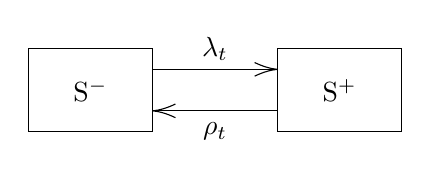
\begin{tikzpicture}[x=0.75pt,y=0.75pt,yscale=-1,xscale=1]
%uncomment if require: \path (0,300); %set diagram left start at 0, and has height of 300

\draw    (160, 120) rectangle (220, 160)   ;
\draw    (280, 120) rectangle (340, 160)   ;
\draw    (220,130) -- (280,130) ;
\draw [shift={(280,130)}, rotate = 180] [color={rgb, 255:red, 0; green, 0; blue, 0 }  ]   (0,0) .. controls (3.31,-0.3) and (6.95,-1.4) .. (10.93,-3.29)(0,0) .. controls (3.31,0.3) and (6.95,1.4) .. (10.93,3.29)   ;

\draw    (220,150) -- (280,150) ;

\draw [shift={(220,150)}, rotate = 0] [color={rgb, 255:red, 0; green, 0; blue, 0 }  ]   (0,0) .. controls (3.31,-0.3) and (6.95,-1.4) .. (10.93,-3.29)(0,0) .. controls (3.31,0.3) and (6.95,1.4) .. (10.93,3.29)   ;

\draw (190,140) node  [align=left] {S$^{-}$};
\draw (310,140) node  [align=left] {S$^{+}$};
\draw (250,120) node  [align=left] {$\lambda_t$};
\draw (250,160) node  [align=left] {$\rho_t$};
\end{tikzpicture}}
    \caption[Reverse catalytic model with constant transition parameters]{Schematic representation of the reverse catalytic model, where individuals transit between seronegative ($\text{S}^-$) and seropositive ($\text{S}^+$) states with age-dependent rates $\lambda_t$ (seroconversion rate) and $\rho_t$ (seroreversion rate).}
    \label{fig:M0}
\end{figure}

The seroconversion rate (SCR or $\lambda_t$) is the annual average rate by which individuals with age $t$ change from seronegative to seropositive, upon malaria infection.
This rate is directly related to transmission intensity and has shown to correlate well with popular epidemiological measures of malaria transmission such as parasite and entomological inoculation rate \cite{corran2007serology, drakeley2005estimating, bodker2003relationship}.
Seroreversion rate (SRR or $\rho_t$) is the annual average rate by which seropositive individuals with age $t$ return to the seronegative state due to antibody decay.
This rate can be influenced by individual characteristics such as age or genetics \cite{corran2007serology}, and be used to predict how many seropositive individuals are expected to remain after complete interruption of transmission \cite{corran2007serology}.
%\\ in the absence of \\
%RECURRENT
%prolonged
%infection 
%The use of these models have the Markov property of lack of memory in a stochastic process, where for time $t$, the probability of transition from one state to another does not depend on previous transitions.This allows for the assumption of a probabilistic restart every time an individual transits from one state to the other.The probability of an individual with age $t$ being at one of the serological states is then defined by a probability matrix
%
%\begin{equation}
%    P(t)=[p_{i|j}(t)], \quad i,j=0,1 ,
%\end{equation}
%
%\noindent where $p_{i|j}(t)$ is the conditional probability of an individual with age $t$ being in state $i$ given he started the process in the state $j$. Making use of these probabilities, the transitional rates can be defined through the transition rate matrix,
%\begin{gather}
%    R = \begin{bmatrix} -\lambda    & \lambda \\ 
%                        \rho        & -\rho \end{bmatrix}
%\end{gather}
%\noindent where $\lambda$ and $\rho$, respectively representing the SCR and SRR, are the transition parameters from one state to the other. The presented negative values for the parameters in the matrix are simply to assure the sum of each line is equal to zero. 

When using RCMs to estimate malaria transmission intensity, one should assume the lower age limit to be $t=1$ year old.
While all individuals are usually assumed to be born seronegative ($\pi_0=0$), when dealing with responses to malaria parasites, the new born's immune system may be influenced by the presence of inherited maternal antibodies.
These antibodies eventually wane over the first months of the newborn's life.
By removing the first year from the analyses, the influence of the maternal antibodies in the model's estimates is expected to be reduced.
% that \textcolor{red}{outsourced} influence is expected to be reduced.
% \textcolor{red}{reduced the maternal antibodies in the analysis.}


%%%%%%%%%%%%%%%%%%%%%%%%%%%%%%%%
\subsubsection{Malaria under stable transmission intensity}

\textcolor{red}{TENHO DE METER QUE $t>0$}
%Following the previous definitions, a RCM that assumes the transitional rates as constant per unit of time $t$ can be created \cite{muench1959catalytic}.
The simplest RCM assumes both SCR and SRR to be constant over time: $\lambda_t =\lambda$ and $\rho_t = \rho$ (Figure \ref{fig:rcm.models}A).
In this situation, all individuals experience equal risk of exposure at all times.
The expected seroprevalence of individuals with age $t$ explained by this model, henceforward denoted M$_0$, is given by
%
\begin{equation}
    \label{eq:M0}
    \pi_{t|\lambda, \rho}=\frac{\lambda}{\lambda+\rho}\left(1-e^{-(\lambda+\rho)t}\right)\ ,
\end{equation}
%
\noindent
where $\lambda \in \rm I\!R_{0}^{+}$ and $\rho \in \rm I\!R_{0}^{+}$.
Both transition rates are expected to be positive, although the possibilities for $\lambda=0$ and $\rho=0$ are included to allow for some particular cases.
A null SCR value can happen if, by any change, a population has experienced transmission interruption.
In that situation any model will predict seroprevalence equal to zero.
A null SRR indicates that all individuals who are exposed and become positively infected \textbf{(SEROPOSITIVE)} will remain so throughout their remaining life.
Model M$_0$ is an increasing function of age that tends exponentially to a plateau given by $\textstyle\frac{\lambda}{\lambda+\rho}$, when $t\rightarrow\infty$.
The derivation of the equation can be found in Section \ref{appendix:M0.derivation} from Appendices.

While not common to use this model in situations of null SCR, it is worth mention that there are situations where SRR can become a rare event.
When this happens, by considering $\rho\rightarrow0$ the model can be rewritten as a traditional complementary log-log model, with resulting formula
%
\begin{equation}
    \label{eq:rcm.cloglog}
    \log[-\log(1-\pi_t)]=\log\lambda+\log t\ .
\end{equation}
%
\noindent
However, this \textcolor{red}{cloglog -- não defini a abreviatura} model is not usually used in malaria research, but has been used to study scenarios where a unique exposure to the disease develops immunisation with resulting permanent seropositive state \cite{hens2012modeling}.

\begin{figure}[th!]
    \center
    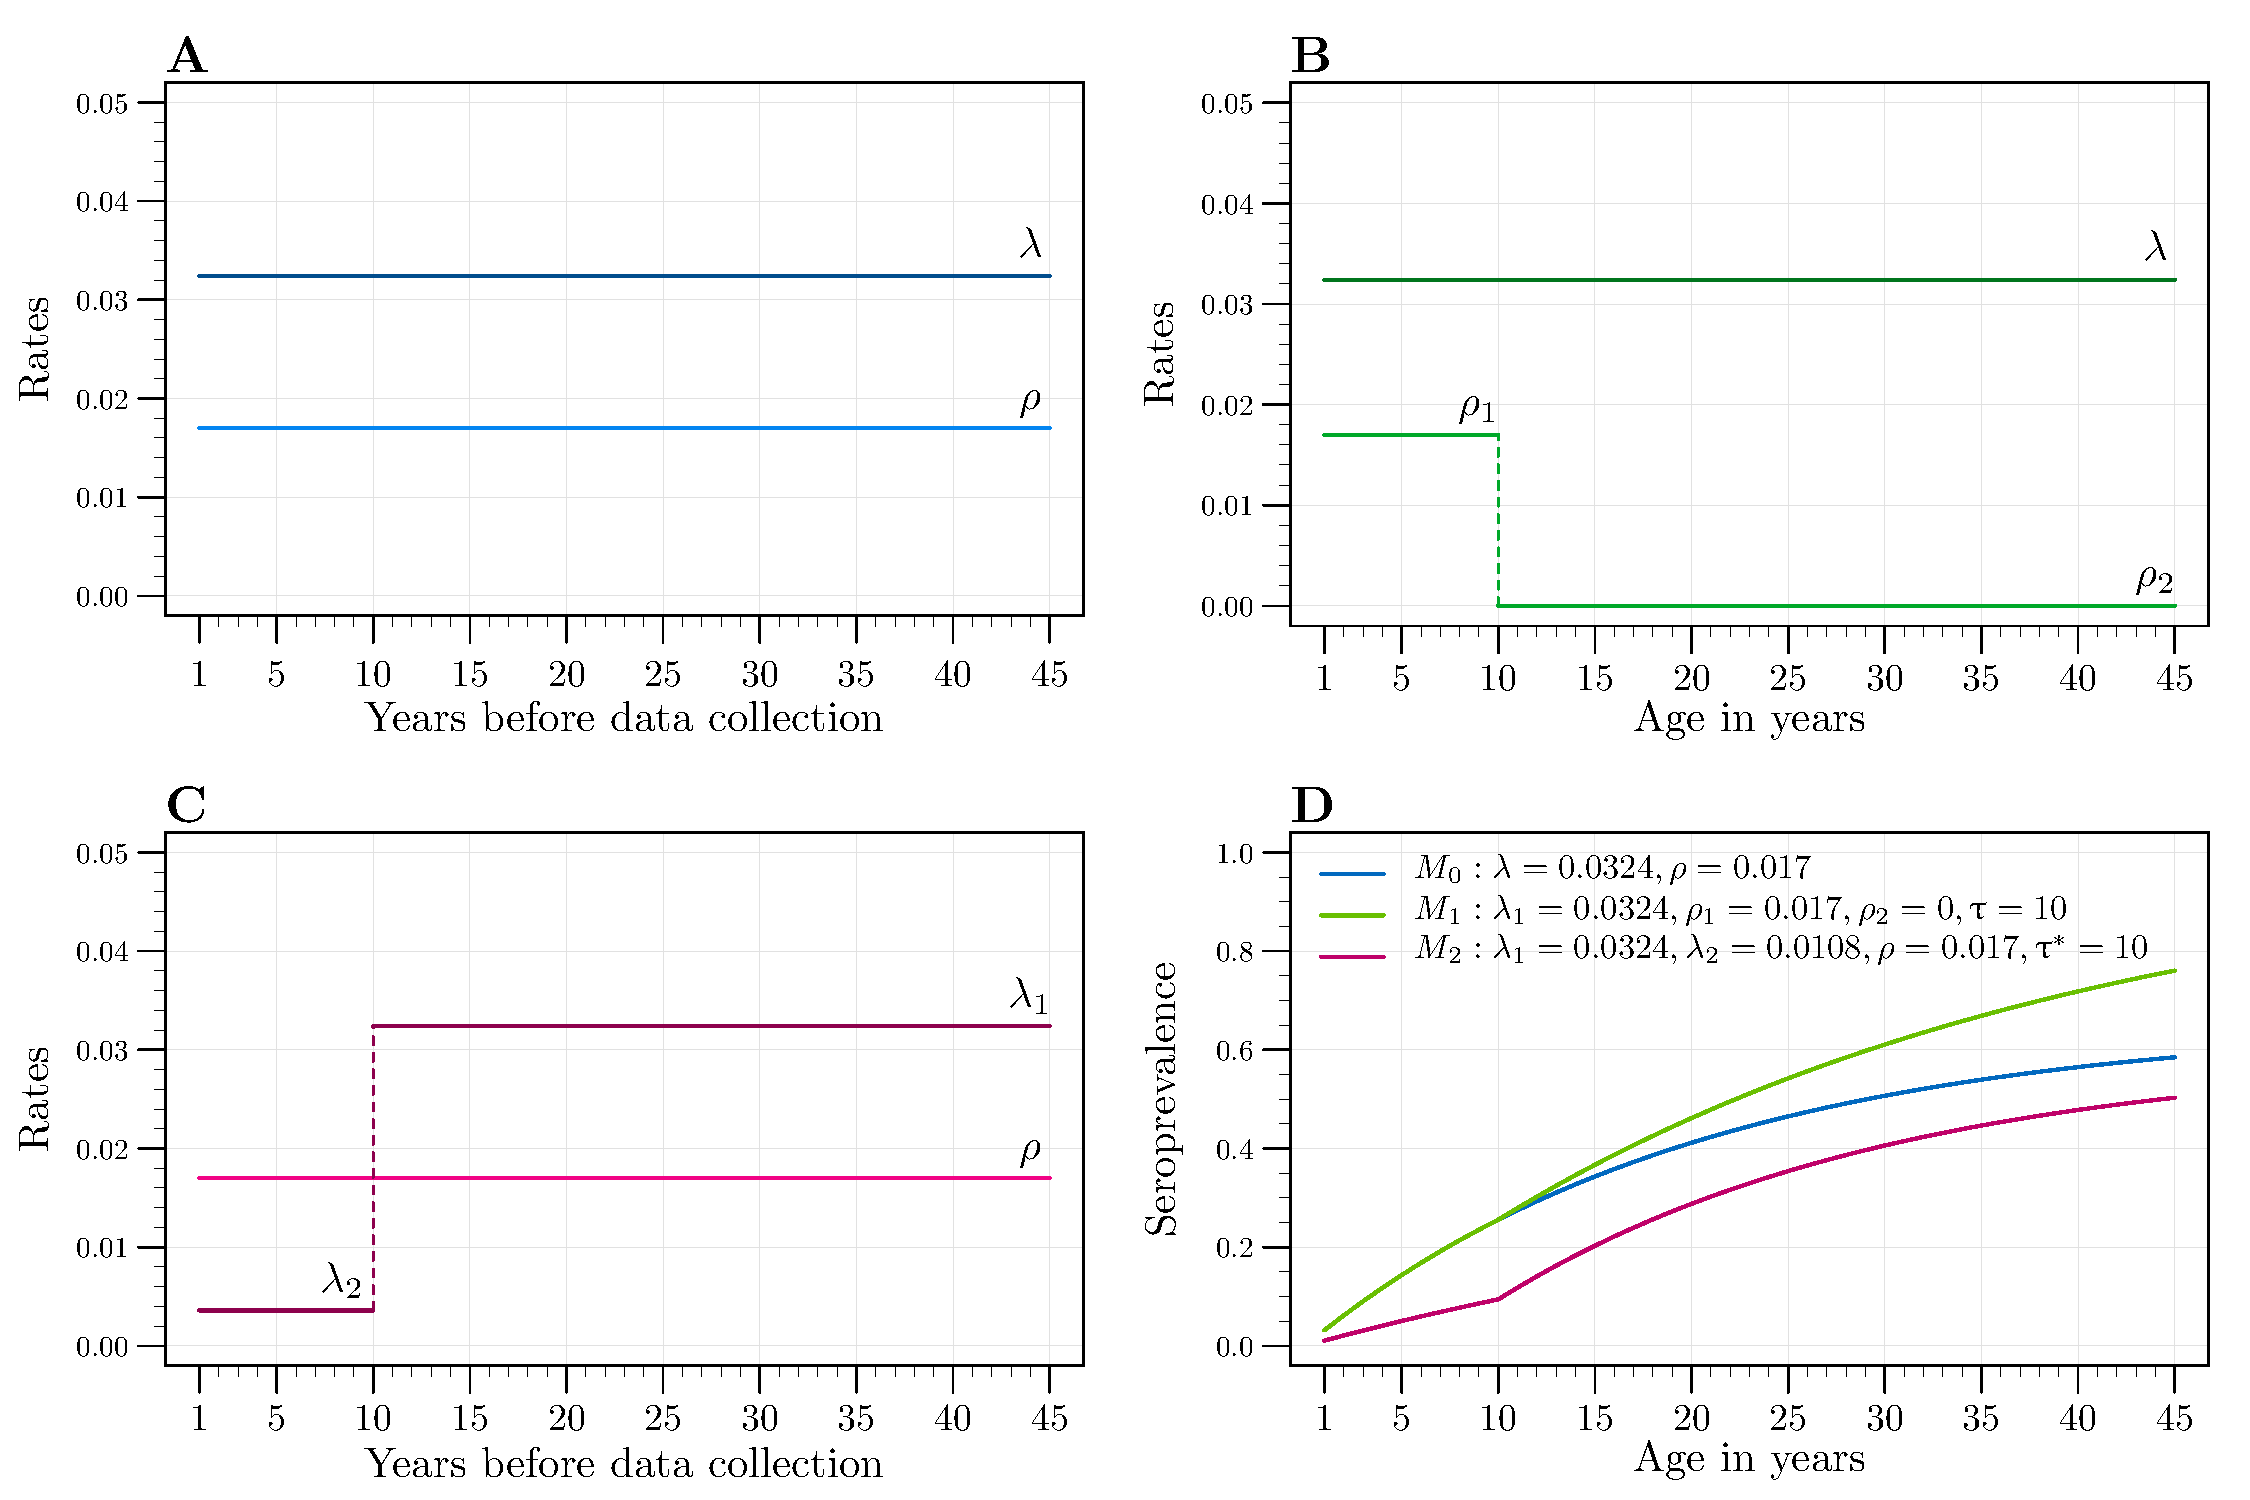
\includegraphics[width=\columnwidth]{images/RCM_structure.pdf}
    \caption[Reverse catalytic models]{Graphical representation of the SCR and SRR for each one of the three RCM described. (\textbf{A}) $\text{M}_0$ with both parameters stable and constant over time; (\textbf{B}) $\text{M}_{1,1}$ that assumes SCR to be constant for all ages and SRR to abruptly decrease to a lower value given an age cutoff $\uptau=10$; and (\textbf{C}) $\text{M}_2$ that assumes SCR to reduce to a lower value, after a change point $\uptau^*=10$. Plot (\textbf{D}) illustrates the resulting age-dependent seroprevalence calculated for each one of the models. \textcolor{red}{It is worth noting that the SRR biphasic behaviour in $\text{M}_{1,1}$ appears to not reflect a visible effect on the seroprevalence, as shown in curve produced by $\text{M}_2$. It may indicate the smaller influence that SRR has in seroprevalence when compared to SCR -- but an influence nonetheless, as $\pi_t$ visibly increases after $\uptau$, when compared to the curve produced by $\text{M}_0$. -- isto posso tirar devido às novas alterações.}}
\label{fig:rcm.models}
\end{figure}


%%%%%%%%%%%%%%%%%%%%%%%%%%%%%%%%
\subsubsection{RCM assuming age-dependent rates to detect heterogeneity in malaria transmission intensity}

%\textbf{aplicar M0}
From a biological point of view, the previous model can be restrictive.
Even in a situation of constant transmission intensity (and thus constant SCR), exposed individuals will eventually develop specific antibodies from an early age, changing SRR over time \cite{cook2011serological}.
%\textbf{because at least SRR can change with age}.
From an epidemiological perspective, considering both rates to be fixed is also limiting.
Model M$_0$ does not account for past actions for control and elimination against the disease that may have occurred, causing SCR to change \cite{cook2010using, sepulveda2015current}.
%\textbf{scr pode mudar devida a intervenções} as modelling serological data under these conditions does not account for acquired immunity over time \cite{cook2011serological} or possible actions for control and elimination against the disease \cite{cook2010using}.
To better represent these two scenarios further mathematical models must be assessed.

In a situation of endemic populations, individuals are expected to gradually develop specific immunity over multiple episodes of infection, throughout their lives \cite{perlmann2002malaria}.
As more individuals become seropositive and remain there due to the constant transmission intensity, over time, less will revert to a seronegative state.
Modelling this effect of acquired immunity should then consider a change in SRR as a function of age.
%that one develops over time can be interpreted as the reduction in SRR over an individual's life, when exposed to stable and constant malaria transmission intensity throughout the hole process.
%The exposure to stable malaria transmission results in a gradual increase of immunological responses, thus individuals that transit to the seropositive state will tend to remain there, adapting to the level of exposure, with consequent antibody waning reduction. 
Mathematically, this \textcolor{red}{variation variação do quê?} can be simplified by modelling all individuals with an initial parameter $\rho_1$ that abruptly changes to a different parameter $\rho_2$ after a specific age cutoff $\uptau$.
The change occur while considering $\lambda_t=\lambda$ (Figure \ref{fig:rcm.models}B).
The age cutoff when such change occurs should vary inversely to the transmission intensity, as individuals that are exposed to high levels of parasite rate are expected to develop specific immunologic responses earlier in life (standard relation between SCR and change in SRR presented in Table \ref{tab:EIR.to.SCR} from Appendices).
%with values between 3 and 5 years in high transmission settings, or values between 15 to 20 years when malaria transmission intensity is lower and requires more time of exposure to adapt.
%for the rest of the individuals' lives 
%This situation is similar to a change due to age-dependent behaviours \cite{}, where mathematically assuming constant SCR, the seroprevalence of an individual aged $t$ years that developed specific immune protection at time $\uptau$ is modelled by the reduction in SRR that follows that instant.
The resulting expected seroprevalence for individuals with age $t$ is explained by model M$_{1,1}$, with formula
%
\begin{equation}
    \label{eq:rcm.reduction.srr}
    \pi_{t | \lambda, \rho_1, \rho_2, \uptau} = \left\{\begin{array}{ll} \frac{\lambda}{\lambda+\rho_{1}}\left(1-e^{-(\lambda+\rho_{1})\uptau}\right)+\frac{\lambda}{\lambda+\rho_{2}}\left(1-e^{-(\lambda+\rho_{2})(t-\uptau)}\right)e^{-(\lambda+\rho_{1})\uptau}\ , & \text{if $t>\uptau$}\\\\  
    \frac{\lambda}{\lambda+\rho_{1}}\left(1-e^{-(\lambda+\rho_{1})t}\right)\ , & \text{if $t\le\uptau$}\ ,\end{array} \right.
\end{equation}
%
\noindent
where $\lambda \in \rm I\!R_{0}^{+}$ is the SCR constant over time, $\rho_1$ the initial SRR that changes to $\rho_2$ given the cutoff $\uptau$.
Similar to M$_{0}$, this function for seroprevalence increases exponentially.

The derivation of this model is based on a RCM presented by Sepúlveda et al. \cite{sepulveda2015current}.
The original model was used to detect an increase in SCR from children and adolescents to adults, due to age-dependent behaviours.
The model proved useful in populations where the male adults go to work on sites that are malaria transmission hotspots, as opposed to younger individuals who stay within the malaria protected housing regions.
\textcolor{red}{Are example -- isto é inglês ali do Pub} some mining populations in the Pará state, near the Brazilian Amazonia \cite{cunha2014serologically}.
% An example are some miner populations near the Brazilian Amazonia where the change in SCR estimated occurs between 25 and 30 years old. This increase in transmission intensity coincides with the age of working miners.
%such as populations where the male individuals are sent to work on sites that are malaria transmission hotspots, as opposed to younger individuals who stay within the treated housing regions \cite{}.
Having a similar structure, model M$_{1,1}$ was created considering a change in SRR instead, assuming SCR to be constant throughout the years.
However, to accurately represent the effect of acquired immunity, the model requires the restriction $\rho_1\geq\rho_2$, where $\rho_1 \in  \rm I\!R_{0}^{+}$ (similar to $\rho$ in M$_0$) and $\rho_2 \in [0,\rho_1]$.

In scenarios of endemic malaria with stable SCR, the constant exposure throughout an individual's life results in a gradual development in specific immunity.
This also indicates the whole population will eventually become seropositive, with SRR reduced to nearly zero by the time an individual reaches adulthood \cite{ondigo2014estimation}.
Based on equation (\ref{eq:rcm.reduction.srr}), this scenario can be represented by an abrupt reduction from $\rho_1 \in \rm I\!R_{0}^{+}$, to $\rho_2=0$, after the age cutoff.
With this model (hereafter denoted M$_{1,2}$) one expects that after a certain age, all seropositive individuals will remain so, with resulting expected seroprevalence closer to 1, as age \textcolor{red}{increases/advances}.
\\
\\

When considering effective interventions for control of endemic malaria, one expects to infer a noticeable reduction in malaria transmission intensity some time before the sampling \cite{cook2010using}.
Mathematically, this reduction can be represented by admitting SCR as a function of time that changes from $\lambda_1$ to $\lambda_2$, given a cutoff $\uptau^*$, and $\rho_t=\rho$ (Figure \ref{fig:rcm.models}C) \cite{sepulveda2015current}.
%This change can be represented with a similar structure to equation (\ref{eq:rcm.reduction.srr}) by admitting a reduction in transmission rate, modulated by a reduction from $\lambda_1$ to $\lambda_2$, given a change point, $\uptau^*$, some time before sample collection (Figure \ref{fig:rcm.models}C) \cite{sepulveda2015current}.
The resulting seroprevalence in this model (hereafter labelled $\text{M}_{2}$) is described  by
%
\begin{equation}
    \label{eq:rcm.reduction.scr}
    \pi_{t| \lambda_1, \lambda_2, \rho, \uptau^*} = \left\{\begin{array}{ll} \frac{\lambda_{2}}{\lambda_{2}+\rho}\left(1-e^{-(\lambda_{2}+\rho)\uptau^{*}}\right)+\frac{\lambda_{1}}{\lambda_{1}+\rho}\left(1-e^{-(\lambda_{1}+\rho)(t-\uptau^*)}\right)e^{-(\lambda_{2}+\rho)\uptau^{*}}\ , & \text{if $t>\uptau^{*}$} \\\\  \frac{\lambda_{2}}{\lambda_{2}+\rho}\left(1-e^{-(\lambda_{2}+\rho)t} \right)\ , & \text{if $t\le\uptau^{*}$}\ , \end{array}\right.
\end{equation}
%
\noindent
where $\lambda_1$ is the initial SCR parameter that abruptly changes to $\lambda_2$ following the age cutoff $\uptau^*$, and $\rho \in \rm I\!R_{0}^{+}$ is the constant and stable SRR.
%Likewise to the previous models, % seroprevalence is also an increasing function of age, reaching a plateau defined by $\textstyle\frac{\lambda_{1}}{\lambda_{1}+\rho}\left(1-e^{-(\lambda_{1}+\rho)\uptau^*} \right)$ when $t\rightarrow\infty$.
Model M$_2$ is published in Sepúlveda et al. Section 2.3.1 \cite{sepulveda2015current}.
%used to assess changes in malaria transmission due to age-dependent cultural behaviours, such as populations where the male adult individuals are sent to work on sites that are malaria transmission hotspots, as opposed to younger individuals who stay within the treated housing regions \cite{}.
When considering successful interventions, a reduction in malaria transmission intensity is assumed, with corresponding reduction in SCR.
With this change in mind, one can expect a reduction after the cutoff through $\lambda_1\geq\lambda_2$, where $\lambda_1 \in \rm I\!R_{0}^{+}$ and $\lambda_2 \in [0,\lambda_1]$.
%The original model was used to describe changes in malaria intensity due to age-dependent behaviours, in situations where having specific characteristics such as age or gender, might influence the rates of malaria transmission intensity, when compared to other groups of the same population. older individuals may have higher malaria transmission intensity when compared to younger individuals of the same population, due to only being exposed in the working sites.

All variations of the RCMs create slightly different age-dependent seroprevalence curves with influence on the maximum reachable plateaus (Figure \ref{fig:rcm.models}D).
Considering the simpler model M$_{0}$ as reference for the curve analysis, the biphasic behaviour of SRR from M$_{1}$ appears to not reflect a visible effect on the expected seroprevalence as does M$_{2}$ considering variation in SCR.
%\textbf{It may indicate the smaller influence that SRR has in seroprevalence -- but an influence nonetheless. Não vale a pena meter}
Model M$_{0}$ is nested within the remaining RCMs, as is model M$_{1,2}$ in M$_{1,1}$.
This relation means the latter models can be transformed into M$_0$ by imposing certain parametric constrains (Figure \ref{fig:lrt.rcm.models}).
This facilitates model comparisons.
%The RCMs applied to serological data are able to estimate malaria transmission intensity even in low transmission settings \cite{corran2007serology}, applying a stochastic analysis and inferring about exposure over time with data from the cross-sectional study.

\begin{figure}[H]
    \center
    \scalebox{1.05}{\tikzset{every picture/.style={line width=0.75pt}} %set default line width to 0.75pt        

\begin{tikzpicture}[x=0.75pt,y=0.75pt,yscale=-1,xscale=1]
%uncomment if require: \path (0,269.6363525390625); %set diagram left start at 0, and has height of 269.6363525390625

\draw    (100, 80) rectangle (160, 120)   ;
\draw    (300, 80) rectangle (360, 120)   ;
\draw    (200, 178.67) rectangle (260, 218.67)   ;
\draw    (160,100) -- (298,100) ;
\draw [shift={(300,100)}, rotate = 180] [color={rgb, 255:red, 0; green, 0; blue, 0 }  ][line width=0.75]    (10.93,-3.29) .. controls (6.95,-1.4) and (3.31,-0.3) .. (0,0) .. controls (3.31,0.3) and (6.95,1.4) .. (10.93,3.29)   ;

\draw    (260,200) .. controls (309.86,199.95) and (329.96,180.35) .. (330,121.79) ;
\draw [shift={(330,120)}, rotate = 449.65] [color={rgb, 255:red, 0; green, 0; blue, 0 }  ][line width=0.75]    (10.93,-3.29) .. controls (6.95,-1.4) and (3.31,-0.3) .. (0,0) .. controls (3.31,0.3) and (6.95,1.4) .. (10.93,3.29)   ;

\draw    (130,120) .. controls (130.07,179.67) and (149.68,199.87) .. (198.51,200) ;
\draw [shift={(200,200)}, rotate = 539.6800000000001] [color={rgb, 255:red, 0; green, 0; blue, 0 }  ][line width=0.75]    (10.93,-3.29) .. controls (6.95,-1.4) and (3.31,-0.3) .. (0,0) .. controls (3.31,0.3) and (6.95,1.4) .. (10.93,3.29)   ;

\draw    (500, 80) rectangle (560, 120)   ;
\draw    (362,100) -- (500,100) ;

\draw [shift={(360,100)}, rotate = 0] [color={rgb, 255:red, 0; green, 0; blue, 0 }  ][line width=0.75]    (10.93,-3.29) .. controls (6.95,-1.4) and (3.31,-0.3) .. (0,0) .. controls (3.31,0.3) and (6.95,1.4) .. (10.93,3.29)   ;

\draw (130,100) node  [align=left] {M$_{1,1}$};
\draw (330,100) node  [align=left] {M$_{0}$};
\draw (230,200) node  [align=left] {M$_{1,2}$};
\draw (230,80) node [scale=0.9]  {$\rho _{1} =\rho _{2}$};
\draw (110,170) node [scale=0.9]  {$\rho _{2} =0$};
\draw (350,170) node [scale=0.9]  {$\uptau  >T$};
\draw (130,70) node [scale=0.7] [align=left] {$p=4$};
\draw (330,70) node [scale=0.7] [align=left] {$p=2$};
\draw (230,230) node [scale=0.7] [align=left] {$p=3$};
\draw (530,100) node  [align=left] {M$_{2}$};
\draw (440,80) node [scale=0.9]  {$\lambda_{1} =\lambda_{2}$};
\draw (440,120) node [scale=0.9]  {$\uptau^* >T$};
\draw (530,70) node [scale=0.8] [align=left] {$p=4$};


\end{tikzpicture}
}
    \caption[Nested reverse catalytic models]{Schematic representation of the different nested RCMs and the possible parametric restrictions that allow one model to transform into another. M$_{1,2}$ is equivalent to M$_{1,1}$ when $\rho_2\neq0$. M$_{0}$ is equivalent to M$_{1,1}$ when $\rho_1\neq\rho_2$, equivalent to M$_{1,2}$ when $\uptau>T$, or equivalent to M$_{2}$ when $\lambda_1\neq\lambda_2$ or $\uptau^*>T$.
    Values of $p$ indicate the number of parameters in each model.}
    \label{fig:lrt.rcm.models}
\end{figure}



%%%%%%%%%%%%%%%%%%%%%%%%%%%%%%%
% INTRO STATISTICAL INFERENCE %
%%%%%%%%%%%%%%%%%%%%%%%%%%%%%%%
\section{Statistical inference}
\label{sec:inference}

Throughout this thesis, analyses were performed within the frequentist framework.
The method of maximum likelihood was applied to estimate the parameters of the described models.
Two distinct approaches were used when estimating the parameters' confidence intervals.
%The profile likelihood approach used to estimate the RCMs with more than two parameters.
Comparisons between the adjusted models were performed by the Akaike's information Criterion (AIC), the Bayesian information criterion (BIC), the log-likelihood ratio test (for nested models), and the area under curve of the receiving operating characteristic (AUC-ROC).
Finally, goodness-of-fit tests were applied to measure the models' adequacy.

%based on the works of Cressie and Read \cite{cressie1984multinomial}.
%As an alternative, the measures of this thesis could have been approached from a Bayesian perspective, although Bayesian methods were not explored.

%%%%%%%%%%%%%%%%%%%%%%%%%%%%%%%
\subsection{Model estimation}

%%%%%%%%%%%%%%%%%%%%%%%%%%%%%%%
\subsubsection{Maximum likelihood estimation}

Parameter estimation was done by maximising equation (\ref{eq:sampling.distribution}) for the sampling distribution.
%For each independent sample of individuals with age $t$, the \textbf{proportion} of positive or seropositive individuals has a Binomial distribution. The joint density of all the observed values (equation (\ref{eq:sampling})) is the likelihood function, $L\left(\boldsymbol{\pi_t} | \boldsymbol{n_t}; \boldsymbol{m_t}\right)$.
In this method, the \textcolor{red}{maximum likelihood estimates (MLE) estimates? Estimators?} are the parameters values that maximise the value of the model's likelihood function based on the observed $m_t$.
Equivalently, one can use the log-likelihood function,
%
%\begin{equation}
%\begin{split}
%\label{eq:mle}
%\log \mathcal{L}(\boldsymbol{\pi_t}|\boldsymbol{n_t},\boldsymbol{m_t}) & =
%\sum_{t=1}^T \log \binom{n_t}{m_t}\pi_t^{\ m_{t}}(1-\pi_t)^{n_t-m_t} \propto \\ 
%& \propto \sum_{t=1}^T n_t\log(1-\pi_t)+m_t\log\left(\frac{\pi_t}{1-\pi_t}\right),
%%\\& \equiv n_t\log [1-\pi_t]+m_t\log \left(\frac{\pi_t}{1-\pi_t}\right).
%\end{split}
%\end{equation}
%\textbf{Esta equação não precisa de ser usada. Se quiser usar tenho de adicionar o índice $k$}\\
%
%\noindent
 transforming all products into sums of the likelihood and thus facilitating the maximisation process \cite{williams1994maximum}.
 %as its maximisation estimators are easier to calculate through the sum of the log-likelihood \cite{williams1994maximum}.
%\textbf{1) maximizar 3.4), usar log porque tranformo produtos em somas}
MLE are calculated by solving the derivative of the log-transformed (\ref{eq:sampling.distribution}) when it is equal to zero.
% \textcolor{red}{ POSSO RETIRAR: The MLE are associated with the regression coefficients $\boldsymbol{\beta}$ that characterise the GLMs and the transitional rates and cutoff parameters in the RCMs, for which the observed sample is more likely to have occurred.}
%Through the properties of the maximum likelihood function,
In theory, such estimators are asymptotically unbiased and jointly normal \cite{casella2002statistical}.
%\textbf{ESTIMATORS} (NUNCA \textbf{PREDICTORS})


%%%%%%%%%%%%%%%%%%%%%%%%%%%%%%%
\subsubsection{Profile likelihood method}

Unknown parameters for the GLMs and model M$_0$ can be estimated via MLE, calculating the likelihood of each value that maximises the overall likelihood function.
\textcolor{red}{For the particular case of...}
RCMs M$_1$ (both variations of the model) and M$_2$ are
age-dependent, with parameters $\uptau$ and $\uptau^*$ defined in years, and restricted within the parametric space $\mathbb{N}^{+}$.
This characteristic makes it difficult to use the simple maximum likelihood estimation.
Knowing that $\uptau$ (although different, for the following description both $\uptau$ and $\uptau^*$ will be broadly described using $\uptau$) can be a sequence of positive natural numbers, the profile likelihood method can be used, varying the natural cutoff value in order to estimate the remaining unknown parameters and its respective likelihood.
The estimation is done by the following steps:
(i) the cutoff parameter $\uptau$ is initially fixed at 1;
(ii) the remaining parameters are estimated via maximum likelihood;
(iii) the corresponding log-likelihood function is calculated at these estimates and;
(iv) $\uptau$ is then increased by one unit of time, repeating steps (ii) and (iii) for every increment until it reaches a predefined maximum age value $T$.
In the end, the overall maximum likelihood estimates are the ones associated with the value of $\uptau$ that provide the maximum value of all the log-likelihood estimates calculated.
%but to estimate all unknown parameters $\{\lambda, \rho_1, \rho_2, \uptau\}$, or $\{\lambda_1, \lambda_2, \rho, \uptau^*\}$, when considering an abrupt reduction in SRR (\ref{eq:rcm.reduction.srr}) or SCR (\ref{eq:rcm.reduction.scr}), respectively, a profile likelihood approach can be applied to the data. In this method, parameter $\uptau$ is defined as a sequence of possible values (years) for when the abrupt reduction may occur, starting at $\uptau=1$ and continuously increasing one unit until an agreed maximum limit value. For each update in sequential change in time $\uptau$, the maximum likelihood estimates for all remaining parameters is calculated, as well as the corresponding log-likelihood function. By the end, the overall maximum likelihood estimates are the ones associated with the value of $\uptau$ that returns the maximum value of all the log-likelihood values.
%Though extremely useful, by using exclusively integer values in the change point value, this profile likelihood method may overestimate the exact moment when the change occurs, even when applied to large sample sizes \cite{sepulveda2015current}. To evaluate their significance as more precise models to study seroprevalence, they must be compared with the model assuming stable rates.

%%%%%%%%%%%%%%%%%%%%%%%%
% CONFIDENCE INTERVALS %
%%%%%%%%%%%%%%%%%%%%%%%%
\subsection{Confidence intervals} \label{seq:confint}

The estimation of the confidence interval for the parameters done in the GLMs was based on properties of the maximum likelihood estimators.
%and the Gauss-Markov theorem 
It assumed estimated coefficients $\hat{{\boldsymbol{\beta}}}$ to be asymptotically normal distributed.
This approach makes use of the most broadly known form of confidence interval estimation, based on the standard error method.
The standard error, $\textstyle\text{se}(\hat{{\beta}})=\sqrt{V(\hat{\beta})}$, is defined as the estimated standard deviation, $\sigma$, a measure of variability of the estimate, that changes its precision based on the sample size.
Since the $\hat{\beta}$ are asymptotic normal distributed, the $100(1-\alpha)$\% confidence intervals can be estimated by calculating the lower and upper limits, given the formula
%
\begin{equation}
    \left(\hat{\beta}\pm \Phi_{\alpha/2} \times \text{se}({\hat{\beta}})  \right)\ ,
    \label{eq:betas.ci}
\end{equation}
%
\noindent
where $\pm \Phi_{\alpha/2}$ represents the lower and upper quantiles of the standard normal distribution, considering tails of size $\alpha/2$.

While working with the RCMs, in some cases the unknown parameters are expected to present estimated values close to zero.
When in these situations, using the standard deviation method to calculate confidence intervals that close to the parametric space margin may not be the most efficient approach.
%In order to estimate the confidence intervals of these parameters,
For this thesis, the proposed alternative is to make use of the likelihood ratio statistic properties by
%Through this comparison method, a poorly estimated likelihood function 
testing null hypotheses for the acceptance or rejection of each one of the estimated parameters, within a defined critic region.
Considering the case of the RCM M$_0$ and the estimation of the confidence interval of parameter $\lambda$.
Via likelihood ratio, the null and alternative hypothesis in these situations are
%
$$H_0:\lambda=\lambda_0\ \textit{vs.}\ H_1:\lambda \neq \lambda_0\text{\ ,}$$
%
where $\lambda$ is the model's parameter and $\lambda_0$ is a defined estimate.
The likelihood ratio statistics is then based on
%
\textcolor{red}{Tenho de meter em coerência com a equação de LRT}
\begin{equation}
    \text{D}=(-2)\times \frac{\Lambda{(\lambda_0,\rho^*)}} {\Lambda{(\hat{\lambda},\hat{\rho})}}\ \overset{a_{\left(\text{H}_0\right)}}{\leadsto}\    \chi_{(1)}^{2}\ ,
\end{equation}
%
\noindent
where $\Lambda{(\lambda_0,\rho^*)}$ is the value of the log-likelihood function under the null hypothesis, with fixed $\lambda_0$ and estimated $\rho^*$, and $\Lambda{(\hat{\lambda},\hat{\rho})}$ is the value of the log-likelihood function under the alternative hypothesis with both parameters $\hat{\lambda}$ and $\hat{\rho}$ equal to the MLE.
%via profile likelihood.
This test statistic is chi-squared distributed under the null hypothesis, with 1 degree of freedom that results from to the difference between the total number of unknown parameters of the models.
The $100(1-\alpha)$\% confidence interval for $\lambda$ is then the range of all possible values of $\lambda$ for which the null hypothesis is not rejected at a given critical region
%equal to or greater than $\text{c}_{\alpha}$.
identified at the level of significance $\alpha$.
This method identifies the confidence intervals as the values for $\lambda$ for which the estimated likelihood ratio test statistic is smaller or equal than the predefined critical value ($\lambda: D\leq \chi^2_{(1)}$).
%This critical region can be \textbf{identified at the 5\% significance} level as the probability of the LRT statistic be equal to or greater than $\text{c}_{\alpha}$.
%The confidence level used was 95\% for a $\alpha=0.05$.
%\textbf{APLICAR NO MODELO M0!!!!}
%Considering the case of the RCM M$_{1,1}$ and parameter $\rho_1$ confidence interval estimation.
%Via likelihood ratio, the null and alternative hypothesis in these situations are 
%$$ H_0:\rho_1=\rho_{1_0}\ \text{vs.}\ H_1:\rho_1 \neq \rho_{1_0}$$
%where $\rho_{1}$ is the model's parameter and $\rho_{1_0}$ is a defined %and instantiated 
%estimate.
%Through the likelihood ratio statistics,
%%
%\begin{equation}
%    \text{LRT}=(-2)\times %\frac{\Lambda_{(\rho_{1_0},\rho_2^*,\lambda^*)}} %{\Lambda_{(\hat{\rho}_1,\hat{\rho}_2,\hat{\lambda})}}\ %\overset{a_{\left(\text{H}_0\right)}}{\leadsto}\    %\chi_{(1)}^{2}
%\end{equation}
%%
%\noindent
%where $\Lambda_{(\rho_{1_0},\rho_2^*,\lambda^*)}$ is the maximum log-likelihood function under the null hypothesis, with fixed $\rho_{1_0}$ and remaining parameters being estimated at each increment of $\uptau$, and $\Lambda_{(\hat{\rho}_1,\hat{\rho}_2,\hat{\lambda})}$ is the estimated maximum log-likelihood function under the alternative hypothesis, with all parameters estimated via profile likelihood.
%This test statistic is chi-squared distributed under the null hypothesis with 1 degree of freedom from to the difference between the total number of parameters in each model.
%\\
%The confidence interval for $\rho_1$ is then the range of all possible values of $\rho_1$ for which the null hypothesis is not rejected at a given critical region $\text{c}_{\alpha}$.
%This critical region can be \textbf{identified at the 5\% significance} level as the probability of the LRT statistic be equal to or greater than $\text{c}_{\alpha}$.
%The confidence level used was 95\% for a $\alpha=0.05$.

%%%%%%%%%%%%%%%%%%%%%%%%%%%%%%%
\subsection{Model comparison}



%%%%%%%%%%%%%%%%%%%%%%%%%%%%%%%
\subsubsection{Information criteria}

The selection of the best fitted models was evaluated using two information criteria: the Akaike's information criterion,
%
\begin{equation}
    \label{eq:aic}
    \text{AIC}=(-2)\times\Lambda_{\text{model}}+2p\ ,
\end{equation}
%
\noindent
and the Bayesian information criterion,
%
\begin{equation}
    \label{eq:bic}
    \text{BIC}=(-2)\times\Lambda_{\text{model}}+p(\log n)\ ,
\end{equation}
%
%Information criteria: AIC (Akaike, 1973) and BIC (Schwarz 1978)
\noindent
%where $\log L(\boldsymbol{\hat{\beta}}|\boldsymbol{m_t})$ is the maximised value for the log-likelihood function for the model with estimated $\boldsymbol{\hat{\beta}}$ parameters, and $k$ the number of parameters considered in said model.
where $\Lambda_{\text{model}}$ is the log-likelihood function evaluated at the MLE for the model under consideration, $p$ is the number of parameters, and $n$ is the sample size.
The first term of the criteria reflects the goodness of fit and the second term describes the model's complexity.
The latter adds a penalty for the number of parameters $p$ included. %, penalising overly complex models.
% overfitting and
%When comparing both CRITERIA, BIC is expected to have an increased penalty value.
%since any sample size $n$ above seven individuals will multiply the number of parameters by a higher value than 2.
Under the principle of parsimony, for a set of candidate models the `best' model is the one presenting the smallest values for AIC or BIC. 



%%%%%%%%%%%%%%%%%%%%%%%%%%%%%%%
\subsubsection{Likelihood ratio test}

The Wilks' likelihood ratio test was used to compare the nested RCMs (see Figure \ref{fig:lrt.rcm.models}).
Under a defined null hypothesis for a parametric constrain, this test indicates the more parsimonious model based on the following test statistic
%
\begin{equation}
    \label{eq:lrt}
    \text{LRT} = (-2)\times(\Lambda_{\text{H}_0} - \Lambda_{\text{H}_1})\   \overset{a_{\left(\text{H}_0\right)}}{\leadsto}\    \chi_{(\Delta p)}^{2}\ ,
\end{equation}
%
\noindent
where $\Lambda_{\text{H}_0}$ and $\Lambda_{\text{H}_1}$ are the estimated maximum log-likelihood functions of the models that characterise the null and alternative hypothesis.
Under the null hypothesis this test statistic is asymptotically chi-squared distributed, $\chi_{(\Delta p)}^{2}$, where $\Delta p$ degrees of freedom is the difference between the total number of parameters from each one of the compared models (subtracting as $\Delta p = p_{H_{1}}-p_{H_{0}}$).
For a significance level fixed at 0.05, p-values $>0.05$ indicate the model defined by the null hypothesis is statistically better than the model represented by the alternative hypothesis.
%is the log-likelihood estimate for the model assuming constant parameters, with stable values for transmission intensity and antibody waning, $\Lambda_{\text{reduction}}$ the log-likelihood estimate for the model assuming abrupt reduction in either SRR or SCR, and $\chi_{(2)}^{2}$ is a Chi-square distribution with two degrees of freedom resulting from the difference in in the total number of parameters for each one of the respective models, $\lambda$ and $\rho$ in the stable model, and either $\lambda$, $\rho_{1}$, $\rho_{2}$ and $\uptau$ in the model with abrupt reduction in SRR, or $\lambda_1$, $\lambda_2$, $\rho$, and $\uptau^*$ in the model with abrupt reduction in SCR. In case of rejection from the null hypothesis (i.e. p-values under 0.05 for a 5\% significance level) there is statistical evidence to accept a proposed change at an estimated time point.
%For the RCM, log-likelihood ratio test is preferred to the likelihood ratio test to derive confidence intervals rather than the likelihood ratio itself because, provided a sample size



%%%%%%%%%%%%%%%%%%%%%%%%%%%%%%%
\subsubsection{Area under the receiver operating characteristic curve}

The receiver operating characteristic (ROC) curve is a standard technique used to infer about the performance of a model by measuring its predictive outcome accuracy \cite{hosmer2013applied}.
This method explores the trade-off between sensitivity and specificity.
These statistical measures are, respectively, the proportion by which a model correctly predicts a true positive or seropositive individual as a case, and the proportion by which it correctly detects a negative or seronegative individual as a non-case.
Using these measures, the accuracy of a model depends on how often, and \textcolor{red}{without mistakes/with wrong predictions}, it differentiates between cases and non-cases.

The ROC curve of a model can be plotted for different cutoff points using the sensitivity values (proportion of identified true cases) in function of $1-\text{specificity}$ (proportion of wrongly identified cases).
The resulting area under the ROC curve (AUC), with range from 0 to 1, can be used as an index for a model's accuracy.
\textcolor{red}{Value 0.5 predicts taht a model is no better than a random guess.}
AUC values equal to 0 indicate a poorly performing model, misidentifying every single individual of a population sample.
Value of 1 indicates a perfectly accurate model that is able of correctly predict the status of all individuals.
When applied to several models under the same conditions, this measure for predictive accuracy can be used as an index statistics for model comparison.



%%%%%%%%%%%%%%%%%%%%%%%%%
% GOODNESS-OF-FIT TESTS %
%%%%%%%%%%%%%%%%%%%%%%%%%
\section{Goodness-of-fit tests}

To assess the goodness-of-fit of the models, several tests were performed inspecting the agreement between the observed and expected values.
The Hosmer-Lemeshow goodness-of-fit statistic was used to assess the fit of the GLMs \cite{hosmer2013applied}.
This test organises the outcomes in bin-like sub-groups $i=(1,\ldots,g)$, based on percentiles of the estimated probabilities called `deciles of risk groups', and with formula given by
%These sub-groups are usually referred to as `deciles of risk groups'.
%
\begin{equation}
    \label{eq:hosmer.lemeshow}
    C_{HL}^2= \sum_{i=1}^g\frac{(M_{i}-n_{i}\hat{\pi}_{i})^2}{n_{i}\hat{\pi}_{i}\left(1-\hat{\pi}_{i}\right)}\ \overset{a_{\left(\text{H}_0\right)}}{\leadsto}\    \chi_{(g-1)}^{2}\ ,
\end{equation}
%
\noindent
where $M_{i}$ and $n_{i}$ are the number of infected or seropositive individuals and the total number of individuals recorded within each decile of risk group $i$, respectively, $\hat{\pi}_{i}$ is the prevalence or seroprevalence for individuals in the decile of risk group $i$.
Under the null hypothesis that the model fits the data well, this test statistic is asymptotically chi-squared distributed, $\chi_{(g-1)}^{2}$, with $g-1$ degrees of freedom.
With the intent to create balanced sample sizes across the deciles of risk groups, this test can create a somewhat arbitrarily subdivision of the observations instead of grouping observations by their respective values of variables, possibly lowering the test's power.
%and producing limited results.
%A large p-value in this test may simply indicate the lack of evidence against the null hypothesis and in favour of the alternative hypothesis.

Assuring that more than a single goodness-of-fit test statistic would be applied, the test proposed by Noel Cressie and Timothy Read \cite{cressie1984multinomial} was used, of formula
%
\begin{equation}
    \label{eq:cressie.read}
    \text{CR}^2 = \frac{2}{\delta(\delta+1)} \sum_{i=1}^g M_i \left[ \left(\frac{M_i}{n_i\hat{\pi}_i}\right)^\delta-1\right]\ \overset{a_{\left(\text{H}_0\right)}}{\leadsto}\    \chi_{(g-1)}^{2}\ ,
\end{equation}
%
%\textbf{COMO É QUE O $p$ É CALCULADO? NUMERO DE GRAUS DE LIBERDADE? NUMERO DE CLASSES?}
\noindent
where $M_i$ and $n_i$ are the number of infected or seropositive individuals and the total number of individuals within a class $i=(1,\dots,g)$, $\hat{\pi}_i$ is the prevalence or seroprevalence for individuals of that group, $\delta \in \rm I\!R$ is a parameter that depending on its attributed value identifies the different goodness-of-fit tests used, and $g$ is the total number of classes considered.
By varying the values of $\delta$ on the equation, the tests here used are the Pearson's $\chi^2$ ($\delta=1$), the log-likelihood ratio statistic ($\delta=0$), the Freeman-Tukey statistic ($\delta=\textstyle-\frac{1}{2}$), the Neyman modified $\chi^2$ statistic ($\delta=-1$), and the modified log-likelihood ratio statistic ($\delta=-2$).
Under the null hypothesis for no difference between the observed and the estimated values, all test statistics are asymptotically chi-squared distributed, $\chi_{(g-1)}^{2}$, with ($g-1$) degrees of freedom.
For a significance level fixed at 0.05, p-values above this limit lead to the non rejection of the hypothesis of equality between the observed frequency distribution and the expected frequencies obtained by the model under testing.
%the recorded infected or seropositive individuals, and the expected numbers 
%
%Under the null hypothesis of equal probabilities, all the proposed tests are asymptotically chi-squared distributed, $\chi_{(\text{p}-1)}^2$, with $\text{p}-1$ degrees of freedom.
%For a significance levels fixed as $5\%$, this hypothesis is rejected for an alternative hypothesis, if the resulting estimated p-value found by use of the $\chi_{\text{p}-1}^2$ expression is greater than or equal to $0.05$.
%Other known alternative tests are then proposed and used, based on the information gathered in the work presented by Noel Cressie and Timothy Read in 1984 \cite{cressie1984multinomial}, where `working rules' are provided to decide which goodness-of-fit test should be used, when considering a Multinomial distribution.
%To test the fitted models, one can infer about the consistency of the calculated probabilities of an individual of age $t$ being positive or seropositive, $\pi_t$, for each model.
%The proposed goodness-of-fit tests are then the most commonly used Pearson's $\chi^2$
%\begin{equation}
%    \label{eq:1.chisquared}
%    X^2=\sum_{t=1}^T \frac{\left(M_t - n_t\pi_t\right)^2}{n_t\pi_t},
%\end{equation}
%\noindent the log-likelihood ratio statistic
%\begin{equation}
%    \label{eq:2.log.LRT.statistic}
%    G^2=2\times\sum_{t=1}^T M_t \log\left(\frac{M_t}{n_t\pi_t}\right),
%\end{equation}
%\noindent the Freeman-Tuckey statistic
%\begin{equation}
%    \label{eq:3.freeman.tuckey}
%    T^2=4\times\sum_{t=1}^T\left[\sqrt{M_t}-\sqrt{n_t\pi_t}\right]^2,
%\end{equation}
%\noindent the Neyman modified $\chi^2$ statistic
%\begin{equation}
%    \label{eq:4.neyman.modified}
%    NM^2=\sum_{t=1}^T \frac{\left(M_t - n_t\pi_t\right)^2}{M_t},
%\end{equation}
%\noindent and the modified log-likelihood ratio statistic
%\begin{equation}
%    \label{eq:5.LRT.modified}
%    GM^2=2\times\sum_{t=1}^T M_t \log\left(\frac{n_t\pi_t}{M_t}\right),
%\end{equation}
%\noindent where for all, $M_t$ is the number of seropositive individuals observed for age $t$, and the multiplication between the total number of individuals with age $t$, $n_t$, with the probability of an individual with that age being seropositive, $\pi_t$, returns the number of expected number of individuals for that age that would be seropositive, based on the values of $\pi_t$ calculated through the different models.
%Under the null hypothesis of equal probabilities, all the proposed tests are asymptotically chi-squared distributed, $\chi_{(\text{p}-1)}^2$, with $\text{p}-1$ degrees of freedom.
%For a significance levels fixed as $5\%$, this hypothesis is rejected for an alternative hypothesis, if the resulting estimated p-value found by use of the $\chi_{\text{p}-1}^2$ expression is greater than or equal to $0.05$.



%%%%%%%%%%%%%%%%%%%%%%%%
% STATISTICAL SOFTWARE %
%%%%%%%%%%%%%%%%%%%%%%%%
\section{Statistical software}

All statistical analyses and inference tests were done in the software R, version 3.4.1.
Maximum likelihood estimates of the regression coefficients in the GLMs were calculated through the command-defined function \texttt{glm()}.
\textcolor{red}{This method uses the iteratively reweighted least squares (IRLS) for the maximum likelihood estimation, where through a process of weighted iteration, the best linear unbiased estimates $\hat{\beta}_0,\hat{\beta}_1,\dots,\hat{\beta}_k$ are found. Isto tem de estar na parte inferencial e não aqui}
These estimated values are the ones which maximise the likelihood.
% minimise the sum of squared deviations of the observations from their expected values.
Their respective confidence intervals were obtained by use of the function \texttt{confint()}.
%There are several numerical techniques which can be used to solve the maximum likelihood equations, such as the Newton-Raphson or Expectation-Maximisation algorithm.

Profile likelihood method to estimate parameters from the RCMs used the \texttt{optim()} function.
For each initialised value of $\uptau$, \texttt{optim()} finds the remaining estimates that maximise the likelihood function associated to the model's equation, through consecutive iterations.
The developments and analyses of the RCMs done in this thesis helped to develop and test the \emph{SERO-AID} package.
This R package (currently in its final stages of development) was created specifically with the intent to facilitate seroprevalence analyses, allowing the comparisons between different RCMs, such as the M$_0$ or M$_2$.